\documentclass{article}

\textwidth=6.5in
\textheight=8.5in
\voffset=-54pt
\oddsidemargin=0in
\evensidemargin=0in
\setlength{\parskip}{8pt}
\setlength{\parindent}{0pt}

\usepackage{amsmath, amssymb}
\usepackage{ifthen}

\usepackage[inline]{enumitem}
\setlist{topsep=0pt, parsep=8pt}

\usepackage[rgb,table]{xcolor}\convertcolorsUfalse
\usepackage{graphicx}

% change hyperref options
\PassOptionsToPackage{hyphens}{url}
\usepackage[bookmarks,colorlinks,linkcolor=black,citecolor=blue,pdfstartview=FitH,urlcolor=blue]{hyperref}
\hypersetup{pdfpagemode=UseNone}
\usepackage{bookmark}

\usepackage{graphicx}
\usepackage{multicol}
\usepackage{framed}
\usepackage{array}

\usepackage{icomma}

\usepackage{pifont}
\newenvironment{noanswer}{}{}
\newlist{altenumerate}{enumerate}{3}

\usepackage{soul}

\usepackage{pgfplots}
\pgfplotsset{compat=1.18}  
\pgfplotscreateplotcyclelist{mycolor}{black, blue, red, green!70!black, magenta, purple, cyan, orange }  
\pgfplotsset{
  disabledatascaling,
  cycle list=tikzcolor, 
  axis lines=middle,
  every axis plot/.style={no marks, thick},
  every axis/.style={
    enlarge x limits=false,
    enlarge y limits=auto,
    xlabel style={at={(current axis.right of origin)},anchor=west},
    ylabel style={at={(current axis.above origin)},anchor=south},
    % extra x and y ticks for asymptotes
    extra x tick style={grid=major, grid style={dashed,black}},
    extra y tick style={grid=major, grid style={dashed,black}},
    /pgf/number format/1000 sep={},
  },    
  tick label style = {font=\footnotesize, fill=\currentbgcolor, inner sep=0pt},    
  xticklabel shift=1pt,    
  scaled ticks=false,
  scaled y ticks=false,
  unbounded coords=jump,
  samples=101,
  minor tick length=0,
  scatter/classes={
    open={mark=*,draw=black,fill=white, mark size=2, thin},
    closed={mark=*,draw=black,fill=black, mark size=2, thin}
  },
  width=3in,
}
\pgfplotsset{open/.style={only marks, mark=*, fill=white, thin, mark size=2}}
\pgfplotsset{closed/.style={only marks, mark=*, draw=black, fill=black,
    thin, mark size=2}}
\pgfplotsset{labeled/.style={nodes near coords, only marks, mark=*, draw=black, fill=black, thin, mark size=2, point meta=explicit symbolic}}

\newcommand{\axes}[1][]{
  \begin{tikzpicture}
    \begin{axis}[xtick=\empty, ytick=\empty, ymin=-2, ymax=2,
      xmin=-4.25, xmax=4.25, #1]
    \end{axis}
  \end{tikzpicture}
}
\usepackage{tikz}
\usetikzlibrary{
  matrix,%
  % enables the snake paths
  decorations.pathmorphing,%
  % enables bigger arrows
  decorations.markings,%
  decorations.pathreplacing,%
  decorations.text,%
  calc,%
  patterns,%
  shapes.geometric,%
  arrows,
  decorations.shapes,
  positioning,
  plotmarks,
  intersections
}
\tikzset{>=latex} % sets default arrow type in tikz
\tikzset{font=\normalsize}
\tikzset{mark size=1.5pt, mark options=thin}
\tikzset{pin distance=4pt,
  every pin edge/.style={<-, thin, shorten <= -2pt}}

\interfootnotelinepenalty=10000
\renewcommand{\thefootnote}{(\arabic{footnote})}

\usepackage{multirow, bigdelim}

% change to \usepackage[sols]{handout} to see solutions
\usepackage{handout}

\providecommand{\check}{}
\renewcommand{\check}{\ifmmode{\text{ \ding{51} }}\else{\ding{51} }\fi}
\definecolor{checkcolor}{rgb}{0.7,0,0}
\newenvironment{checkanswer}{\color{checkcolor}\check}{\color{black}}  

\newcommand\iscurrentenumi[1]{%
  \ifthenelse{\equal{#1}{\theenumi}}{}{#1}}
\setenumerate[1]{ref=\#\arabic*}
\setenumerate[2]{ref=\protect\iscurrentenumi{\theenumi}(\alph*)}
\newcommand\enumiiprefix[2]{%
  \ifthenelse{{\equal{#1}{\theenumi}}\AND{\equal{#2}{(\alph{enumii})}}}{}{}%
  \ifthenelse{{\equal{#1}{\theenumi}}\AND{\NOT{\equal{#2}{(\alph{enumii})}}}}{#2}{}%
  \ifthenelse{\equal{#1}{\theenumi}}{}{#1#2}%
}
\setenumerate[3]{ref=\protect\enumiiprefix{\theenumi}{(\alph{enumii})}\roman*}

\makeatletter

% underline links               
\let\@href=\href
\renewcommand{\href}[2]{\@href{#1}{\ul{#2}}}

\newdimen\SOUL@dimen %new
\def\SOUL@ulunderline#1{{%
    \setbox\z@\hbox{#1}%
    % \dimen@=\wd\z@
    \SOUL@dimen=\wd\z@ %new
    \dimen@i=\SOUL@uloverlap
    \advance\SOUL@dimen2\dimen@i %\dimen@ exchanged too
    \rlap{%
      \null
      \kern-\dimen@i
      % \SOUL@ulcolor{\SOUL@ulleaders\hskip\dimen@}%
      \SOUL@ulcolor{\SOUL@ulleaders\hskip\SOUL@dimen}% new
    }%
    \unhcopy\z@
  }}

\makeatother

\newcommand{\related}[1]{%
\fcolorbox{black}{yellow}{%
  %\parbox[t]{12pt}{$\clubsuit$}%
  \parbox[t]{\linewidth-8pt}{\emph{Related problems:} #1}}}

\renewcommand{\answer}[1]{#1}

\definecolor{purple}{rgb}{0.5,0,1.0}
\definecolor{hotpink}{rgb}{1, 0, 0.5}

\definecolor{skyblue}{rgb}{0, 0.5, 1}

\newcommand{\goal}[1]{\textbf{\textcolor{skyblue}{#1}}}
\newcommand{\indvar}[1]{\textbf{\textcolor{hotpink}{#1}}}

\usepackage{amsthm}

% make URLs print in the same font
\usepackage{url}
\urlstyle{same}

\usepackage{pifont}
\def\exend{\hfill\ding{118}}

%\makeatletter\@addtoreset{equation}{section}\makeatother
%\renewcommand{\theequation}{\arabic{section}.\arabic{equation}}

\newtheoremstyle{theorem}% name
{8pt}%      Space above
{0pt}%      Space below
{\itshape}%         Body font
{}%         Indent amount (empty = no indent, \parindent = para indent)
{\bfseries}% Thm head font
{.}%        Punctuation after thm head
{.5em}%     Space after thm head: " " = normal interword space;
                                %       \newline = linebreak
{}%         Thm head spec (can be left empty, meaning `normal')

\theoremstyle{theorem}

\let\Theorem\undefined
\newtheorem{Theorem}[equation]{Theorem}
\let\Definition\undefined
\newtheorem{Definition}[equation]{Definition}
\let\Summary\undefined
\newtheorem{Summary}[equation]{Summary}
\let\Conjecture\undefined
\newtheorem{Conjecture}[equation]{Conjecture}
\let\Fact\undefined
\newtheorem{Fact}[equation]{Fact}

\renewcommand{\thesubsection}{\arabic{subsection}}
\makeatletter
\def\@seccntformat#1{\@ifundefined{#1@cntformat}%
   {\csname the#1\endcsname\quad}%       default
   {\csname #1@cntformat\endcsname}}%    enable individual control
\newcommand\section@cntformat{}
\makeatother

  \usepackage{exam}

\usepackage{fancyhdr}
\lhead{\textcolor{white}{This content is protected and may not be shared, uploaded, or distributed.}}
\rhead{}
\rfoot{\vspace*{\fill}\footnotesize\textcopyright{} \emph{Harvard Math Ma}}
\renewcommand{\headrulewidth}{0pt}
\pagestyle{fancy}
\begin{document}

  \title{Exam 1, Practice 1}

\instructions{instructions.tex}{}

\listofproblems

\begin{enumerate}
\item \label{fall2018-premidterm-practice3-4} \points{14} 

  From May 2014 to August 2014, the median price of a two bedroom home in Cambridge \textbf{increased at an increasing rate}. Let $C(t)$ be the median cost, in thousands of dollars, of a two bedroom home in Cambridge $t$ months after January 1, 2014.

  Suppose that, at the beginning of May ($t = 4$), the median cost of a two bedroom home in Cambridge was \$514,000. By the beginning of August ($t=7$), the median cost was \$580,000.

  \solonly{\related{\href{https://people.math.harvard.edu/~jjchen/mathma/docs/homework/PS09.html}{Problem Set 9}, {{\#4}}}}

  \begin{enumerate}
  \item \label{fall2018-premidterm-practice3-4a}

    \begin{problem}[\vfill]
      Sketch a possible graph of $C(t)$ on the interval $[4, 7]$, labeling the coordinates of any points you know. (Please make a large sketch, as you will add to it in later parts of this problem.) 
    \end{problem}

    \begin{solution} 
      Since we're told that the price was increasing at an increasing rate, the graph is increasing and concave up. 
      \begin{center}
        \answer{
          \begin{tikzpicture}
            \begin{axis}[axis x discontinuity=parallel, axis y discontinuity=parallel, xlabel={$t$ (months)}, ylabel={cost (thousands of dollars)}, xmin=3, ymin=500, clip=false]
              \addplot+[domain=4:7] {(1474 - 11*x + 7*x^2)/3}; %
              \addplot+[closed] coordinates {(4, 514)} node[below]{(4, 514)}; 
              \addplot+[closed] coordinates {(7, 580)} node[right]{(7, 580)}; 
            \end{axis}
          \end{tikzpicture}
        }
      \end{center}
    \end{solution} 

  \item \label{fall2018-premidterm-practice3-4b}
    \begin{problem}[\vfill\newpage]
      What was the average rate of change of the median cost of a two-bedroom home in Cambridge from $t=4$ to $t = 7$? Please include units in your answer.
    \end{problem}

    \begin{solution}
      $\displaystyle \dfrac{C(7) - C(4)}{7-4} = \frac{580-514 \text{ thousand dollars}}{3 \text{ months}} = \boxed{22 \text{ thousand dollars/month}}$.
    \end{solution} 

  \item
    \begin{problem}[\vfill]
      Use a secant line to approximate the median cost of a two bedroom home in Cambridge on May 16, 2014 ($t = 4.5$). Can you determine whether your estimate is an overestimate or an underestimate? Explain your reasoning clearly and completely, and illustrate on your graph in \ref{fall2018-premidterm-practice3-4a}.
    \end{problem}

    \begin{solution}
      We only know two points on this graph, so there's only one secant line we're able to find, the one between $(4, 514)$ and $(7, 580)$. We found in \ref{fall2018-premidterm-practice3-4b} that this line has slope 22, so its equation is $C - 514 = 22 (t - 4)$, or $C = 22 (t - 4) + 514$. The height of this line at $t = 4.5$ is $22 (0.5) + 514 = 525$, so our estimate is \fbox{\$525,000}. The secant line lies above the graph at $t = 4.5$, so this is an \fbox{overestimate}:
      \begin{center}
        \begin{tikzpicture}
          \begin{axis}[axis x discontinuity=parallel, axis y discontinuity=parallel, xlabel={$t$ (months)}, ylabel={cost (thousands of dollars)}, xmin=3, ymin=500, clip=false]
            \addplot+[domain=4:7] {(1474 - 11*x + 7*x^2)/3}; %
            \addplot+[closed] coordinates {(4, 514)} node[below]{(4, 514)};% 
            \addplot+[closed] coordinates {(7, 580)} node[right]{(7, 580)};%
            \addplot+[skyblue, samples=2] coordinates { (4, 514) (7, 580) };%
            \addplot+[closed, skyblue] coordinates {(4.5, 525)} node[anchor=south east]{$(4.5, 525)$}; %
          \end{axis}
        \end{tikzpicture}
      \end{center}
    \end{solution} 

  \item
    \begin{problem}[\vfill\newpage]
      Suppose that, at the beginning of May, the median price of a two bedroom home in Cambridge was increasing at an instantaneous rate of \$15,000 per month. Use this information to estimate the median price of a two bedroom home in Cambridge on May 16, 2014. Can you determine whether your estimate is an overestimate or an underestimate? Explain your reasoning clearly and completely, and illustrate on your graph in \ref{fall2018-premidterm-practice3-4a}.
    \end{problem}

    \begin{solution}      
      If the price is changing at a rate of \$15000 per month, in half a month, we expect it to increase by about (\$15000 / month)(0.5 months) = \$7500, so the expected price on May 16 is $514,000+7,500 = \boxed{\$521,500}$.

      Graphically, \$15,000 is the slope of the tangent line at $t = 4$, and our estimate is the height of the tangent line at $t = 4.5$. Since this tangent line lies under the graph, our estimate is an \fbox{underestimate}:
      \begin{center}
        \begin{tikzpicture}
          \begin{axis}[axis x discontinuity=parallel, axis y discontinuity=parallel, xlabel={$t$ (months)}, ylabel={cost (thousands of dollars)}, xmin=3, ymin=500, clip=false]
            \addplot+[domain=4:7] {(1474 - 11*x + 7*x^2)/3}; %
            \addplot+[closed] coordinates {(4, 514)} node[below]{(4, 514)};% 
            \addplot+[closed] coordinates {(7, 580)} node[right]{(7, 580)};%
            \addplot+[hotpink, samples=2] coordinates { (4, 514) (5, 529) };%
            \addplot+[closed, hotpink] coordinates {(4.5, 521.5)} node[anchor=north west]{$(4.5, 521.5)$}; %
          \end{axis}
        \end{tikzpicture}
      \end{center}
    \end{solution}

  \end{enumerate} 

\item \label{fall2015-1a-fpractice2-1} \points{7} 

  \begin{enumerate}
  \item \label{definition-of-derivative-visualization}
    \begin{problem}[\vfill]
      Below is the graph of a function $f$, with a value $a$ marked.
      Explain how to visualize $f'(a)$ on this graph.

      \begin{tikzpicture}
        \begin{axis}[xtick={1}, xticklabels={$a$}, ytick=\empty, ymin=-2, 
          ymax=4, width=2.5in]
          \addplot+[domain=-2:2] {x^3-x+1};
          \solonly{\addplot+[domain=0.75:1.25, red]{2*(x-1)+1};}
        \end{axis}
      \end{tikzpicture}
    \end{problem}

    \begin{solution}
      $f'(a)$ is the slope of the tangent line at $x = a$; that is, it's
      the slope of the red line shown above.
    \end{solution}

  \item \label{definition-of-derivative}
    \begin{problem}[\vfill]
      State the limit definition of $f'(a)$.
    \end{problem}

    \begin{solution}
      We could write this as $f'(a) = \boxed{ \lim_{h \to 0} \frac{f(a + h) - f(a)}{h} \text{ or } \lim_{x \to a} \frac{f(x) - f(a)}{x - a}}$.

      The variable we use in the limit can be called anything; for example, we could also write the limits above as $f'(a) = \displaystyle \lim_{\clubsuit \to 0} \frac{f(a + \clubsuit) - f(a)}{\clubsuit}$ and $f'(a) = \displaystyle \lim_{q \to a} \frac{f(q) - f(a)}{q - a}$. 
    \end{solution}

  \item
    \begin{problem}[\nstretch{4}]
      Your roommate doesn't understand why the definition you gave in
      \ref{definition-of-derivative} expresses the quantity you drew in
      \ref{definition-of-derivative-visualization}.  Explain what the
      definition is saying and why it exactly gives the quantity you drew
      in \ref{definition-of-derivative-visualization}.
    \end{problem}

    \begin{solution}
      The idea of the definition is to first look at secant lines from
      $(a, f(a))$ to nearby points.  If we have a nearby point $(x, 
      f(x))$, then the secant line between $(a, f(a))$ and $(x, f(x))$
      looks like this: 
      \begin{center}
        \begin{tikzpicture}
          \begin{axis}[xtick={1, 1.5}, xticklabels={$a$, $x$}, ytick=\empty, ymin=-2, 
            ymax=4, width=2.5in]
            \addplot+[domain=-2:2] {x^3-x+1};
            % \addplot+[domain=0.75:1.25, red]{2*(x-1)+1};
            \addplot+[domain=1:1.5, blue]{15/4*(x-1)+1};
          \end{axis}
        \end{tikzpicture}        
      \end{center}
      This line has slope $\dfrac{f(x) - f(a)}{x - a}$.  As we let the
      nearby point approach $(a, f(a))$, this slope approaches $f'(a)$, so
      $f'(a) = \displaystyle \lim_{x \to a} \frac{f(x) - f(a)}{x - a}$.

      If we instead called the nearby point $(a + h, f(a + h))$, then the
      secant line would have slope $\dfrac{f(a + h) - f(a)}{h}$:
      \begin{center}
        \begin{tikzpicture}
          \begin{axis}[xtick={1, 1.5}, xticklabels={$a\vphantom{h}$, $a + h$}, ytick=\empty, ymin=-2, 
            ymax=4, width=2.5in]
            \addplot+[domain=-2:2] {x^3-x+1};
            % \addplot+[domain=0.75:1.25, red]{2*(x-1)+1};
            \addplot+[domain=1:1.5, blue]{15/4*(x-1)+1};
          \end{axis}
        \end{tikzpicture}        
      \end{center}
      In this case, the way to have the point $(a + h, f(a + h))$ approach
      $(a, f(a))$ is to have $h$ approach 0, so $\displaystyle \lim_{h \to
        0} \frac{f(a + h) - f(a)}{h}$ gives the slope of the tangent
      line. 
    \end{solution}

  \end{enumerate}

\item \label{fall2017-premidterm-5} \points{22}  %Justin

  Let $f(x) = \dfrac{3}{x+1} - 2$.

  \begin{enumerate}

  \item \label{fall2017-premidterm-5a}
    \begin{problem}[\vfill]
      Sketch the graph of $f(x)$. Label any intercepts and asymptotes with their exact coordinates, and explain how you found them. 

      \probonly{\axes[width=10cm, height=10cm]}        
    \end{problem}

    \begin{solution}
      We start with $y = \dfrac{1}{x}$, shift it left by 1 unit, stretch it vertically by 3, and shift it down by 2. This moves the asymptotes to $x = -1$ and $y = -2$. To find the $x$-intercept, we solve
      \begin{align*}
        \frac{3}{x + 1} - 2 &= 0 \\
        \frac{3}{x + 1} &= 2 \\
        \frac{3}{2} &= x + 1 \\
        \frac{1}{2} &= x 
      \end{align*}
      The $y$-intercept is $f(0) = \dfrac{3}{1} - 2 = 1$. So, here's the labeled graph:
      \begin{center}
        \answer{
          \begin{tikzpicture}
            \begin{axis}[ xmin=-5.5, xmax=5.5, ymin=-5.5, ymax=5.5, width=10cm, height=10cm, xtick={0.5, -1}, ytick={1, -2}]
              \addplot [domain=-5.5:-1] {3/(x+1)-2}; %
              \addplot [domain=-1:8] {3/(x+1)-2}; %
              \addplot [dashed, domain=-8:8] {-2}; %
              \addplot [dashed] coordinates {(-1, -8) (-1, 8)}; %
            \end{axis}
          \end{tikzpicture}
        }
      \end{center}
    \end{solution}

  \item
    \begin{problem}[\stretch{0.5}]
      What's the domain of $f$? 
    \end{problem}

    \begin{solution}
      The domain is all real numbers except $x=-1$, or $\boxed{(-\infty, -1)\cup(-1, \infty)}$.
    \end{solution}

  \item
    \begin{problem}[\nstretch{0.5}]
      What's the range of $f$?
    \end{problem}

    \begin{solution}
      The range is all real numbers except $y=-2$, or $\boxed{(-\infty, -2)\cup(-2, \infty)}$. 
    \end{solution}

  \end{enumerate}

  \probonly{We're still working with $f(x) = \dfrac{3}{x+1} - 2$.}

  \begin{enumerate}[resume]
  \item \label{fall2017-premidterm-5-deriv}
    \begin{problem}[\stretch{4}]
      Use the limit definition of the derivative to compute $f'(x)$.
    \end{problem}

    \begin{solution} 
      \begin{align*}
        f'(x)&=\lim_{h\to 0}\frac{f(x+h)-f(x)}{h}\\
        &= \lim_{h \to 0} \frac{1}{h} \Big[ f(x + h) - f(x) \Big] \\
        &=\lim_{h\to 0} \frac{1}{h} \left[\left(\frac{3}{x+h+1}-2\right)-\left(\frac{3}{x+1}-2\right)\right]\\
        &=\lim_{h\to 0} \frac{1}{h} \left(\frac{3}{x+h+1}-\frac{3}{x+1}\right) \\
        &=\lim_{h\to 0} \frac{1}{h} \left(\frac{3}{x+h+1} \cdot \frac{x + 1}{x + 1} -\frac{3}{x+1} \cdot \frac{x + h + 1}{x + h + 1} \right) \\
        &=\lim_{h\to 0} \frac{1}{h} \left(\frac{3(x+1)-3(x+h+1)}{(x+h+1)(x+1)}\right) \\
        &=\lim_{h\to 0} \frac{1}{h} \left( \frac{3x+3-3x-3h-3}{(x+h+1)(x+1)}\right) \\
        &=\lim_{h\to 0} \frac{1}{h} \frac{-3h}{(x+h+1)(x+1)}\\
        \intertext{When we take the limit as $h \to 0$, we're looking only at $h \neq 0$, so $\left( \frac{1}{h} \right) h = 1$. (If $h = 0$, then $\left( \frac{1}{h} \right) h$ would be undefined.)}%
        &=\lim_{h\to 0}\frac{-3}{(x+h+1)(x+1)} \\
        \intertext{Now that we no longer have the $\frac{1}{h}$, the expression is defined when $h = 0$, so we can just plug in $h = 0$:} %
        &=\frac{-3}{(x+0+1)(x+1)} \\
        &=\boxed{-\frac{3}{(x+1)^2}}
      \end{align*}
    \end{solution}

  \end{enumerate}

  % rest added by Janet in 2023

  Suppose $g$ is a function with domain $(0, \infty)$ that is continuous on its domain and has $g'(x) = \dfrac{3}{x + 1} - 2$.

  \begin{enumerate}[resume]
  \item
    \begin{problem}[\vfill]
      Where is $g$ increasing? Where is $g$ decreasing?
    \end{problem}

    \begin{solution}
      We can answer this by looking at the sign of $g'$. Looking at the graph we drew in \ref{fall2017-premidterm-5a} (and remembering that we currently only care about the interval $(0, \infty)$, since that's what we were told the domain of $g$ is), $g'$ is positive on the interval $(0, 0.5)$ and negative on $(0.5, \infty)$. So, $g$ is \fbox{increasing on $(0, 0.5)$ and decreasing on $(0.5, \infty)$}.
    \end{solution}

  \item
    \begin{problem}[\vfill\newpage]
      Where is $g$ concave up? Where is $g$ concave down?
    \end{problem}

    \begin{solution}
      We can answer this by looking at where $g'$ is increasing or decreasing.
      Looking at the graph we drew in \ref{fall2017-premidterm-5a}, we see that $g'$ is always decreasing on $(0, \infty)$, so $g$ is \fbox{concave down on $(0, \infty)$}.

      We could also answer this by making a sign chart for $g''(x)$, which we calculated in \ref{fall2017-premidterm-5-deriv}. 
    \end{solution}

  \item \label{fall2017-premidterm-5-antideriv}

    \begin{problem}[\stretch{3}]
      Sketch a possible graph of $g$. 
    \end{problem}

    \begin{solution}
      We want to sketch a graph that's increasing and concave down on $(0, 0.5)$ and decreasing and concave down on $(0, 0.5)$. Here's one possibility: 
      \begin{center}
        \answer{
          \begin{tikzpicture}           
            \begin{axis}[xtick={0.5}, ytick=\empty]
              \addplot+[domain=0.01:4] {3*ln(x + 1) - 2*x + 2}; 
            \end{axis}
          \end{tikzpicture}
        }
      \end{center}
      Since we aren't given any additional information about $g$, any vertical shift of this would also be correct. 
    \end{solution}

  \item
    \begin{problem}[\vfill\newpage]
      Do we have enough information to determine how many zeros ($x$-intercepts) $g$ has? Explain. 
    \end{problem}

    \begin{solution}
      \fbox{No}. Since we only know $g'$, any vertical shift of the graph we sketched is also a possible graph of $g$. We can see that a vertical shift of the graph we sketched in \ref{fall2017-premidterm-5-antideriv} could have 0, 1, or 2 zeros. 
    \end{solution}

  \end{enumerate}

\item \points{6} 

  Here's the graph of a function $f$:
  \begin{center}
    \begin{tikzpicture}[declare function={f(\x)=1000 + (-3 - \x)*(-11 + \x)*(-7 + \x)*(-5 + \x)*(-3 + \x)*\x;}]
      \begin{axis}[disabledatascaling=false, xtick={1.18152, 3.9624, 5.8}, xticklabels={$a$, $b$, $c$}, ytick=\empty]
        \addplot+[domain=-0.25:7.25]{f(x)}; %
        \draw[dashed, thin, gray] (axis cs: 1.18152, 0) -- (axis cs: 1.18152, {f(1.18152)}); %
        \draw[dashed, thin, gray] (axis cs: 3.9624, 0) -- (axis cs: 3.9624, {f(3.9624)}); %
        \draw[dashed, thin, gray] (axis cs: 5.8, 0) -- (axis cs: 5.8, {f(5.8)}); %
      \end{axis}
    \end{tikzpicture}
  \end{center}
  In each part, fill in the blank with ``$<$'', ``$=$'', or ``$>$''. No explanation is necessary.
  \begin{enumerate}
  \item
    \begin{problem}
      $f(a)\;\cfitb{0.25in}{<}\;f(b)$
    \end{problem}

    \begin{solution}
      We can see that $f(a)$ is negative while $f(b)$ is positive. 
    \end{solution}

  \item
    \begin{problem}
      $f'(a)\;\cfitb{0.25in}{=}\;f'(b)$
    \end{problem}

    \begin{solution}
      Both $f'(a)$ and $f'(b)$ are 0 (the tangent line at each point has slope 0). 
    \end{solution}

  \item
    \begin{problem}
      $\dfrac{f(b) - f(a)}{b - a} \cfitb{0.25in}{>} \dfrac{f(a) - f(c)}{a - c}$ 
    \end{problem}

    \begin{solution}
      $\dfrac{f(b) - f(a)}{b - a}$ is the slope of the secant line between $(a, f(a))$ and $(b, f(b))$ (shown in pink below) while $\dfrac{f(a) - f(c)}{a - c}$ is the slope of the secant line between $(c, f(c))$ and $(a, f(a))$ (shown in blue below).
      \begin{center}
        \begin{tikzpicture}[declare function={f(\x)=1000 + (-3 - \x)*(-11 + \x)*(-7 + \x)*(-5 + \x)*(-3 + \x)*\x;}]
          \begin{axis}[disabledatascaling=false, xtick={1.18152, 3.9624, 5.8}, xticklabels={$a$, $b$, $c$}, ytick=\empty]
            \addplot+[domain=-0.25:7.25]{f(x)}; %
            \draw[dashed, thin, gray] (axis cs: 1.18152, 0) -- (axis cs: 1.18152, {f(1.18152)}); %
            \draw[dashed, thin, gray] (axis cs: 3.9624, 0) -- (axis cs: 3.9624, {f(3.9624)}); %
            \draw[dashed, thin, gray] (axis cs: 5.8, 0) -- (axis cs: 5.8, {f(5.8)}); %
            \addplot+[sharp plot, hotpink] coordinates {(1.18152, {f(1.18152)}) (3.9624, {f(3.9624)}) }; % 
            \addplot+[sharp plot, skyblue] coordinates {(1.18152, {f(1.18152)}) (5.8, {f(5.8)}) }; % 
          \end{axis}
        \end{tikzpicture}
      \end{center}
      Both slopes are positive, and the pink slope is steeper, so it's more positive than the blue slope. Therefore, the pink slope is greater. 
    \end{solution}
  \end{enumerate}

  In the remaining parts, fill in the blank with ``$<$'' or ``$>$''. Again, no explanation is necessary.

  \begin{enumerate}[resume]
  \item
    \begin{problem}
      $f''(a) \cfitb{0.25in}{>} 0$
    \end{problem}

    \begin{solution}
      The graph is concave up at $x = a$.
    \end{solution}

  \item
    \begin{problem}
      $f''(b) \cfitb{0.25in}{<} 0$
    \end{problem}

    \begin{solution}
      The graph is concave down at $x = b$.
    \end{solution}

  \item
    \begin{problem}[\newpage]
      $f''(c) \cfitb{0.25in}{>} 0$
    \end{problem}

    \begin{solution}
      The graph is concave up at $x = c$.
    \end{solution}

  \end{enumerate}

\item \label{fall2018-midterm-6} \points{14} 
  % Rosalie

  Penny has a farm in Western Massachusetts where she grows pumpkins and squashes. She sells each pumpkin for \$3 and each squash for $\$$1. However, the amount of land needed for each fruit is different: each pumpkin requires one square foot of land to grow, but one square foot of land is enough for 5 squashes to grow.

  Penny has 500 square feet of land available to grow her fruits. She needs to decide how much of the land to allocate to pumpkins and how much to allocate to squashes for the coming season. She is going to use all 500 square feet and will only plant pumpkins and squashes.

  \begin{enumerate}
  \item \label{fall2018-midterm-6a}

    \begin{problem}[\newpage]
      Write a function $R(p)$ that describes the revenue Penny will make from selling her pumpkins and squashes, as a function of the area $p$ she allocates for pumpkins. (Assume that Penny is able to sell everything she grows.)

      Make sure to communicate your reasoning clearly. 
    \end{problem}

    \begin{solution}
      We'll use the same general strategy as in {{\#3}} on \href{https://people.math.harvard.edu/~jjchen/mathma/docs/worksheets/worksheet06-sols.html}{the worksheet ``Function Composition, Modeling with Functions''}: 
      \begin{noanswer}
        \begin{enumerate}[label=\arabic*.]
        \item \hl{\textbf{Understand the Problem.}}

          \hl{\textbf{Goal:}} Express \goal{revenue} as a function of \indvar{$p$ (area for growing pumpkins)}.

        \item Since our goal is \goal{revenue}, let's \hl{\textbf{write a formula}} for it, \hl{\textbf{defining any variables we use}}.
          \begin{align*}
            \goal{$R$} &= \text{revenue from pumpkins} + \text{revenue from squash} \\
            \intertext{Each pumpkin is worth \$3 and each squash is worth \$1, so we can rewrite this as:}
            &= 3(\text{number of pumpkins sold}) + 1(\text{number of squash sold}) \\
            \intertext{Each square foot of land can be used to produce 1 pumpkin or 5 squash, so we can rewrite this again as:} &= 3 (1p) + \ (5s) \text{ where $s = \text{area Penny allocates to growing squash}$}
          \end{align*}

        \item Now, we need to \hl{\textbf{relate the variables we've used}} ($s$ and $p$) so that we can get everything in terms of the desired variable (\indvar{$p$}). To do this, we must \hl{\textbf{use something else we know about the situation}}. We're told that Penny has 500 square feet of land. Since she is using all of it, we must have $p + s = 500$, so $s = 500 - p$. Substituting this into our equation above, we get $\goal{$R$} = 3p + 5(500-p) = \boxed{2500-2p}$.
        \end{enumerate}
      \end{noanswer} \answeronly{$2500 - 2p$}
    \end{solution}

  \item
    \begin{problem}[\vfill]
      What is the domain of your function from \ref{fall2018-midterm-6a}?
    \end{problem}

    \begin{solution}
      The domain consists of all sensible values of $p$. Based on the constraint coming from Penny's available land, she could plant no pumpkins ($p=0$) or 500 square feet of pumpkins ($p=500$) or anything in between. So the domain of $R(p)$ is $\boxed{[0, 500]}$.
    \end{solution}

  \item
    \begin{problem}[\vfill]
      What is the range of your function from \ref{fall2018-midterm-6a}?
    \end{problem}

    \begin{solution}
      Since $R(p)$ is a linear equation with domain $[0, 500]$, the range will be every value between $R(0)=2500$ and $R(500)=1500$. So, the range is $\boxed{[1500, 2500]}$.
    \end{solution}

  \item
    \begin{problem}[\vfill\newpage]
      How much area should Penny allocate to pumpkins to earn the most revenue? 
    \end{problem}

    \begin{solution}
      The graph of $R(p)$ looks like this:
      \begin{center}
        \begin{tikzpicture}
          \begin{axis}[xtick={500}, ytick={1500, 2500}, xlabel=$p$, ylabel=$R$, ymin=0, enlarge x limits=auto, width=2in]
            \addplot+[domain=0:500] {2500-2*x};
          \end{axis}
        \end{tikzpicture}
      \end{center}
      So, $R(p)$ is greatest when $p = 0$. Therefore, Penny should allocate \fbox{0 square feet} to pumpkins. (That is, she should only plant squash.)  

      \begin{checkanswer}
        Does this answer make sense? Yes, because each square foot of squash translates to \$5 for Penny, but each square foot of pumpkins is only \$3 for Penny.
      \end{checkanswer}
    \end{solution}
  \end{enumerate}

\item \label{fall2018-premidterm-practice3-6} \points{10} 

  \begin{problem}[\newpage]
    Here's the graph of a function $f$. % modified by Janet to make continuous
    \begin{center}
      \begin{tikzpicture}
        \begin{axis}[ytick=\empty]
          \addplot+[domain=-4:1] {x^4-17*x^2+16}; %
          \addplot+[domain=1:3] {10.5*(x-1)}; %
          \addplot+[domain=3:6] {21}; %
        \end{axis}
      \end{tikzpicture}
    \end{center}
    Sketch the graph of $f'$ on $(-4, 6)$. 
  \end{problem}

  \begin{solution} 
    \begin{center}
      \answer{
        \begin{tikzpicture}
          \begin{axis}[ytick=\empty]
            \addplot+[domain=-4:1, very thick]  {4*x^3-34*x}; %
            \addplot+[domain=1:3, very thick]  {10.5}; %
            \addplot+[domain=3:6, very thick]  {0}; %
            \addplot[open]  coordinates{(1, -30)}; %
            \addplot[open] coordinates{(1, 10.5)}; %
            \addplot[open] coordinates{(3, 0)}; %
            \addplot[open] coordinates{(3, 10.5) (6, 0) (-4, -120)}; %
          \end{axis}
        \end{tikzpicture}
      }
    \end{center}
    We've drawn unfilled dots at $x = -4$ and $x = 6$ to indicate that we were only asked to sketch the graph of $f'$ on the open interval $(-4, 6)$.

    If you're not sure why this is right, play around with \href{https://www.geogebra.org/m/kf3dw5kw}{this applet} (grab the yellow dot and drag it along the graph of $f$).
  \end{solution} 

\item \label{fall2013-1a-midterm1-7}
  \points{7} \finishexam  % Janet

  Some runners wear weight vests while running to get more of a workout. Suppose Tyson goes for a daily two-mile run, and $T(w)$ gives the time (in minutes) it takes him to complete the run when wearing $w$ pounds of extra weight.

  \solonly{\related{{{\#4}} on \href{https://people.math.harvard.edu/~jjchen/mathma/docs/worksheets/worksheet10-sols.html}{the worksheet ``The Derivative Function''}; {{\#1}} on \href{https://people.math.harvard.edu/~jjchen/mathma/docs/worksheets/worksheet11-sols.html}{the worksheet ``Functions and their Derivatives''}; \href{https://people.math.harvard.edu/~jjchen/mathma/docs/homework/PS11.html}{Problem Set 11}, {{\#5}}; \href{https://people.math.harvard.edu/~jjchen/mathma/docs/workshops/workshop04.html}{Workshop 4}, {{\#3}}}}

  \begin{enumerate}
  \item
    \begin{problem}[\vfill]
      What are the units of $T'(w)$?
    \end{problem}

    \begin{solution}
      The units of $T'(w) = \dfrac{dT}{dw}$ are the units of $T$ (time, in minutes) over the units of $w$ (pounds). That is, the units are \fbox{minutes per pound}.

      If you prefer to think graphically, remember that we visualize the derivative at a point as the slope of a line tangent to the graph of $T$. Even though we don't know what the graph of $T$ looks like, the axes should be:
      \begin{center}
        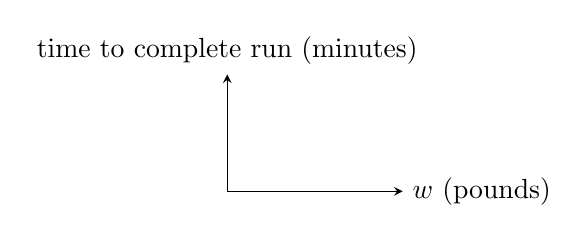
\begin{tikzpicture}
          \begin{axis}[xmin=0, xmax=30, ymin=0, ymax=20, axis equal image,
            ytick=\empty, xtick=\empty, xlabel=$w$ (pounds), ylabel=time
            to complete run (minutes), width=1.5in]
          \end{axis}
        \end{tikzpicture}
      \end{center}
      So, a slope on this graph should have units of minutes per pound. 
    \end{solution}

  \item
    \begin{problem}[\vfill]
      Should $T'(w)$ be positive or negative?  Why?
    \end{problem}

    \begin{solution}
      An increase in weight should result in a longer time to run the 2 miles, so $T'(w)$ should be \fbox{positive}. (A positive change in weight results in a positive change in time.)

      Another way to think about this is to think about the graph of $T(w)$: it should be increasing because higher weight corresponds to longer time. Therefore, the tangent lines of the graph should all have positive slope.
    \end{solution}

  \item Given that $T'(15) = 2$, which of the following statements is most reasonable? Please circle your answer and give a brief explanation (a sentence or two).

    \begin{altenumerate}[label=\protect\maybecircle{\Alph*.}]
    \plainitem If Tyson wears 2 more pounds of weight, then he should complete his run in about 15 minutes.

    \plainitem If Tyson wears 15 pounds of weight, his run should take about 2 more minutes than if he wore no weight at all.

    \circleitem \label{fall2013-1a-midterm1-7-answer} If Tyson increases the amount of weight he wears from 15 to 16 pounds, then his running time should increase by about 2 minutes.

    \plainitem If Tyson increases the amount of weight he wears by 15 pounds, then his running time should increase by about 2 minutes.

    \end{altenumerate}

    \pspace{\vfill}

    \begin{solution}
      The fact that $T'(15) = 2$ means that, when $w = 15$ pounds, the instantaneous rate of increase in Tyson's running time is $2$ minutes per pound. This means that if he increases his weight by one pound, he should expect to take $2$ extra minutes on his run.
      \answeronly{C}
    \end{solution}

  \item
    \begin{problem}[\stretch{0.5}]
      Let $f(t)$ be the weight, in pounds, that Tyson decides to wear for his run $t$ days after September 1. How long does his run on September 8 take? Express your answer in function notation.
    \end{problem}

    \begin{solution}
      Since September 8 is 7 days after September 1, the weight that Tyson wears on September 8 is $f(7)$ pounds. We need to plug this weight into $T$ to get the amount of time it takes him to complete the run, so his run that day takes \fbox{$T(f(7))$ minutes}. 
    \end{solution}

  \end{enumerate}

\end{enumerate}

\end{document}
